\documentclass[a4paper]{article}
\usepackage[utf8]{inputenc}
\usepackage[slovene]{babel}
\usepackage{graphicx}
\usepackage{hyperref}
\usepackage[nottoc]{tocbibind}
\usepackage{caption}
\usepackage{subcaption}
\usepackage{amsmath}
\usepackage{ dsfont }
\usepackage{siunitx}
\usepackage{multimedia}
\usepackage[table,xcdraw]{xcolor}
\usepackage{float}
\setlength\parindent{0pt}

\newcommand{\ddd}{\mathrm{d}}
\newcommand\myworries[1]{\textcolor{red}{#1}}
\newcommand{\Dd}[3][{}]{\frac{\ddd^{#1} #2}{\ddd #3^{#1}}}

\begin{document}
\begin{titlepage}
    \begin{center}
        
\includegraphics[]{logo.png}
        \vspace*{3cm}
        
        \Huge
        \textbf{Numerična minimizacija}
        
        \vspace{0.5cm}
        \large
        3. naloga pri Modelski Analizi 1

        \vspace{4.5cm}
        
        \textbf{Avtor:} Marko Urbanč (28232019)\ \\
        \textbf{Predavatelj:} prof. dr. Simon Širca\ \\
        \textbf{Asistent:} doc. dr. Miha Mihovilovič\ \\
        
        \vspace{2.8cm}
        
        \large
        24.2.2023
    \end{center}
\end{titlepage}
\tableofcontents
\newpage
\section{Uvod}
Numerično minimizacijo poznamo tudi pod širšim imenom matematična optimizacija.
V zelo preprostih pojmih gre za izbito najbolj primernega elementa iz neke množice, 
glede na podane kriterije. Običajno je ta množica neka funkcija, ki jo želimo minimizirati.
Kriterij pa je podan z neko funkcijo, ki nam pove kako dober je neki element. Če se to sliši
zelo podobno kot uvod pri prejšnji nalogi, kjer smo si pogledali Linearno programiranje, je to
zato, ker je to v bistvu ista stvar. Razlika je le v tem, da je pri linearnem programiranju
funkcija, ki jo minimiziramo linearna, pri numerični minimizaciji pa je ta funkcija lahko
poljubna. \\

Z največjim veseljem bi napisal še kakšen bolj matematičen uvod, ampak to bi pomenilo, da bi 
se moral spustiti v podrobnosti delovanja posameznih optimizacijskih algoritmov, kar pa je
precej obsežna tema, še sploh če bi se želel dotakniti vseh, ki sem jih poskusil, ker jih je
res veliko. \\

Veliko problemov se prevede na optimizacijske probleme, zato je to zelo pomembna tema. Če 
ne drugega, je dandanes strašno priljubljeno strojno učenje, ki je v bistvu nič drugega kot
optimizacija neke funkcije, ki nam pove kako dobro se nek model prilega podatkom. Tu se pojavi 
poanta, ki sem jo želel (a neuspešno) povedati v prejšnji nalogi. Optimizacija funkcije z npr. 40 
parametri je zelo malo. V praksi smo zmožni optimizirati funkcije z več milijoni parametrov in tu
se vmeša meni priljubljen High Performance Computing in to da sem želel pri prejšnji nalogi 400k
dimenzij. Tukaj sicer ne bomo počeli tega, ne ker ne bi želel, ampak ker žal nisem utegnil. \\

\section{Naloga}
Naloga je sestavljena iz dveh delov. Poglejmo:
\subsection{Thomsonov problem}
Thomsonov problem je problem, kjer želimo najti najboljšo porazdelitev n točk po sferi, tako da
bo potencial (lahko si mislimo kot električni potencial) čim manjši. To je v bistvu problem, ki
ga rešujemo pri modeliranju atomov. Naloga želi, da za različne metode optimizacije preštudiramo
pojav in natančnost rešitev. \\

\subsection{Vožnja skozi semafor}
Vrača se primer, ki smo ga imeli za prvo nalogo pri Modelski Analizi 1 z to razliko, da bomo tokrat 
namesto variacijskega problema reševali optimizacijski problem. Lagrangian je potrebno zapisati v 
primerni obliki, nato pa lahko uporabimo neko metodo optimizacije, da dobimo rešitev. \\

\section{Opis reševanja}
Reševanja sem se, kot je navada, lotil v Pythonu. Za optimizacijo sem uporabil knjižnico \texttt{scipy},
ki vsebuje veliko različnih metod za optimizacijo. Poskušal sem tudi z komercialnim solverjem \texttt{gurobipy}
do katerega sem dobil dostop v kontekstu prejšnje naloge, ampak nisem dosegel željenih rezultatov. Ideja
je bila, da bi potem reševanje paraleliziral. Poleg tega sem pa uporabil praktično stalen nabor knjižnic, ki
torej \texttt{numpy}, \texttt{matplotlib}, \texttt{pandas} etc. \\

\subsection{Suite of benchmarks}
Za primerjavo uspešnosti različnih metod globalne optimizacije sem definiral suito funkcij, ki so posebej
patološke oz. primerne za testiranje kvalitete optimizacijskih metod. Pogledal sem si:
\begin{itemize}
    \item Basin Hopping
    \item Differential Evolution
    \item Dual Annealing
    \item Simplicial Homology Global Optimization (SHGO)
\end{itemize}

Predstavljeno v enem stavku, Basin Hopping deluje tako, da delamo lokalno optimizacijo, nato pa naključno 
spreminjamo parametre in ponovimo postopek. Differential Evolution je evolucijski algoritem, ki deluje tako,
da naključno generira populacijo, nato pa jo spreminja z nekimi pravili. Dual Annealing je algoritem, ki
deluje na principu simuliranega ohlajanja. SHGO pa je algoritem, ki deluje tako, da razdeli prostor parametrov
na simplicialne komplekse in nato v vsakem izvede lokalno optimizacijo. Podrobneje je SHGO opisan v članku
\cite{Endres2018}. \\

Funkcije, ki sem jih definiral sem 
narisal na slikah (\ref{fig:benchmarks}, \ref{fig:benchmarks2}, \ref{fig:benchmarks3}). Performance metod
pri njihovi optimizaciji je prikazan v rezultatih.\\

\begin{figure}[H]
    \centering
    \makebox[\textwidth][c]{%
    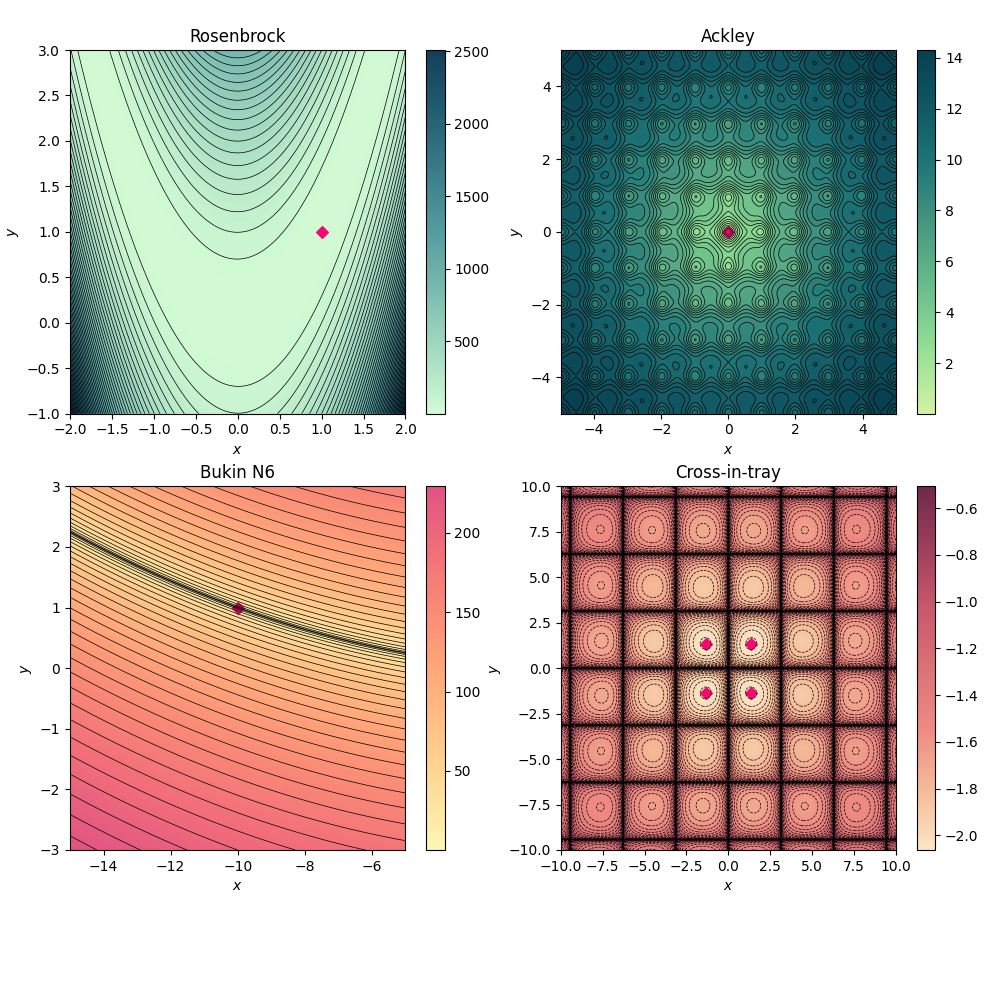
\includegraphics[width=1\textwidth]{../Images/benchmark_1.png}
    }
    \caption{Prve 4 funkcije iz suite of benchmarks.}
    \label{fig:benchmarks}
\end{figure}

\begin{figure}[H]
    \centering
    \makebox[\textwidth][c]{%
    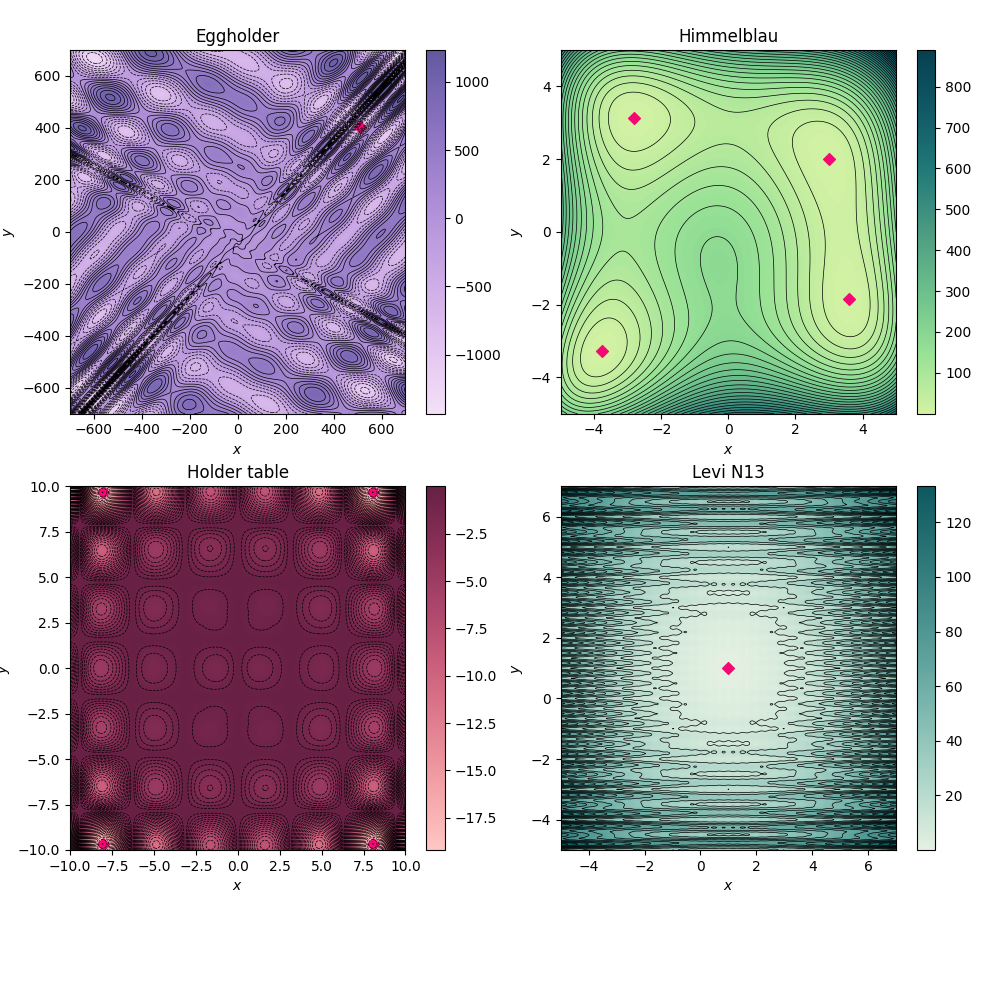
\includegraphics[width=1\textwidth]{../Images/benchmark_2.png}
    }
    \caption{Naslednje 4 funkcije iz suite of benchmarks.}
    \label{fig:benchmarks2}
\end{figure}

\begin{figure}[H]
    \centering
    \makebox[\textwidth][c]{%
    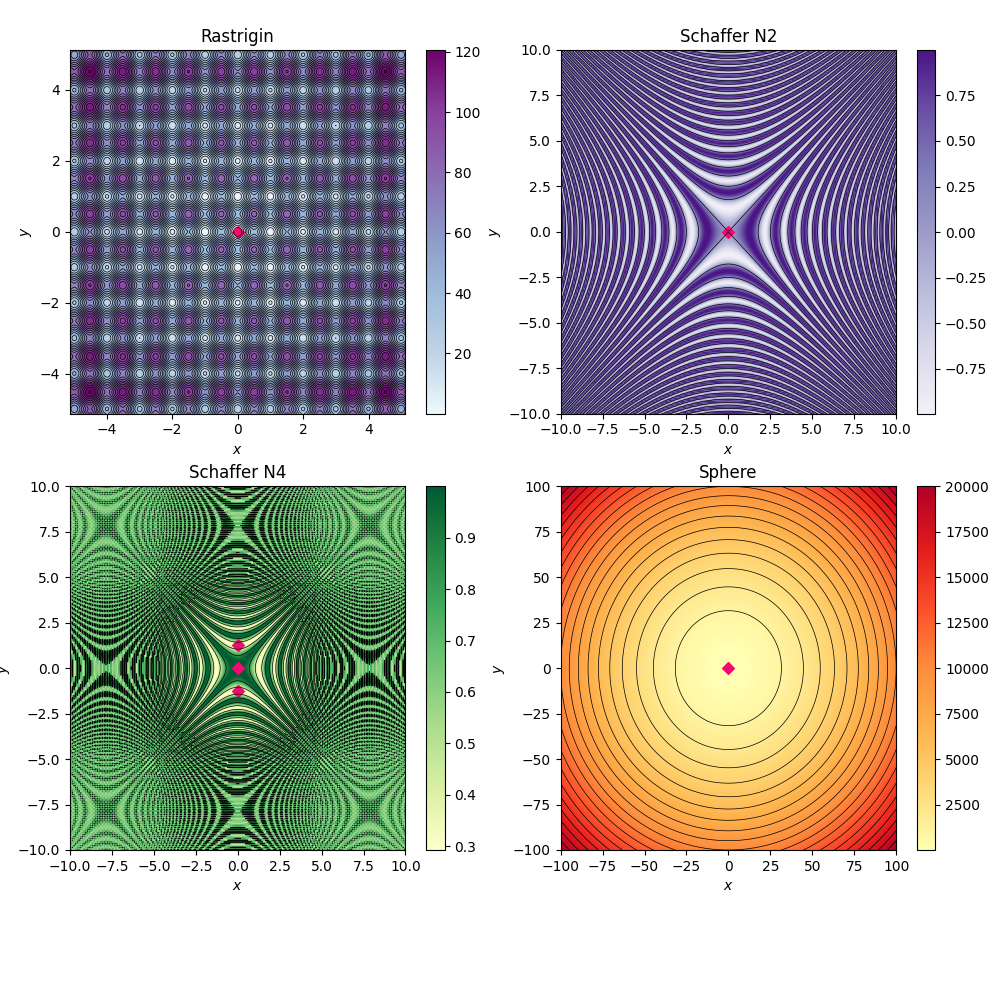
\includegraphics[width=1\textwidth]{../Images/benchmark_3.png}
    }
    \caption{Zadnje 4 funkcije iz suite of benchmarks.}
    \label{fig:benchmarks3}
\end{figure}

\subsection{Thomsonov problem}
Najprej sem napisal funkcijo, ki je za dobljene kote $\theta$ in $\phi$ na enotski sferi izračunala
potencial. Pri temu sem upošteval, da imamo pravzaprav $m = n - 1$ točk, ker je ena točka fiksna. Njo
sem postavil na severni pol. Preostale točke sem porazdelil enakomerno po ekvatorju. Pogledal sem si
natančnost različnih metod, ki jih nudi \texttt{scipy.optimize.minimize()} pri $m=1$, kajti to je edini
primer za katerega sem se počutil samozavestno, da poznam analitičen odgovor. To pomeni, da sta dva naboja 
na krogli, kar pomeni, da gre ne fiksirani naboj v drug pol. Nato sem si pogledal še nekaj primerov 
in naredil animacijo za $m=9$. \\

\subsection{Vožnja skozi semafor}
Najprej sem napisal funkcijo $f(v_0,\>v_1,\>v_2,\>...,\>v_n)$ po trapeznem pravilu, definirano takole:

\begin{equation}
        f =
        \frac{1}{2} \left(\frac{v_1 - v_0}{\Delta t}\right)^2 + \left(\frac{v_2 - v_1}{\Delta t}\right)^2
        + ... + \left(\frac{v_{n-1} - v_{n-2}}{\Delta t}\right)^2 + \frac{1}{2} \left(\frac{v_n - v_{n-1}}{\Delta t}\right)^2\>,    
\end{equation}

kjer je $v_0$ začetna hitrost, $v_n$ končna hitrost, $v_i$ hitrost v $i$-tem trenutku, $\Delta t$ pa časovni korak.
Tej funkciji sem še prištel vez s katero sem zahteval, da je ploščina pod grafo enaka $l$, kjer je $l$ razdalja 
do semaforja. Vez $g(v_0,\>v_1,\>v_2,\>...,\>v_n)$ je definirana takole:

\begin{equation}
    g = 1 + \exp\left[\kappa\left(\frac{1}{2}v_0 + v_1 + ... + v_{n-1} + \frac{1}{2}v_n - 
    \frac{l}{\Delta t}\right)\right]\>.
\end{equation}

Skupno funkcijo sem minimiziral z metodami za lokalno optimizacijo, ki jih ponuja \texttt{scipy.optimize.minimize()}.
Ker sem imel od prvega dela naloge največ uspega z \texttt{Powell} metodo, sem se odločil, da jo uporabim tudi tukaj.
Začetne pogoje sem nastavil tako, da so vse hitrosti enake in tako sem dobil neke rezultate. Bi si pa želel, da bi 
posvetil lahko več časa temu delu naloge, ker se bi mi zdelo zanimivo primerjati bolj podrobno dobljeno z rezultati
prve naloge pri Modelski Analizi 1. Žal je oddajni rok že tu. Lahko si pa pogledamo s kakšno funkcijo imamo opravka.
Na sliki (\ref{fig:semafor}) je prikazana funkcija, ki jo minimiziramo. \\

\begin{figure}[H]
    \centering
    \makebox[\textwidth][c]{%
    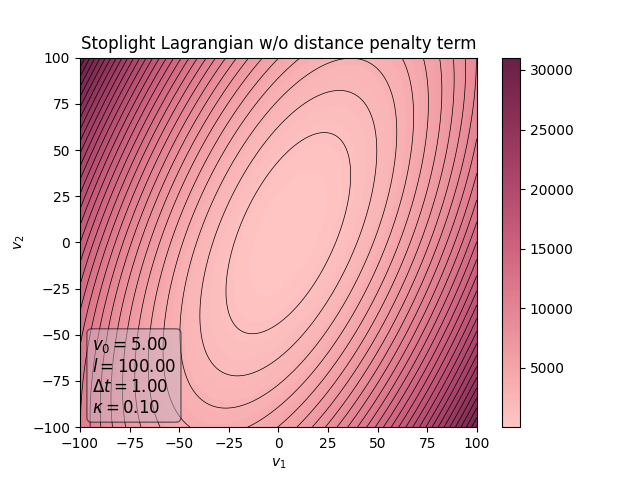
\includegraphics[width=0.8\textwidth]{../Images/stoplight_lagrangian_bare.png}
    }
    \caption{Funkcija, ki jo minimiziramo.}
    \label{fig:semafor}
\end{figure}

\section{Rezultati}
\subsection{Suite of benchmarks}
Kot sem že omenil, sem za primerjavo uspešnosti različnih metod globalne optimizacije definiral suito funkcij, ki so
posebej patološke oz. primerne za testiranje kvalitete optimizacijskih metod. Nato sem si pogledal, za koliko odstopajo
rezultati od pravih vrednosti. Rezultat je prikazan na sliki (\ref{fig:benchmarks_results}). \\

\begin{figure}[H]
    \centering
    \makebox[\textwidth][c]{%
    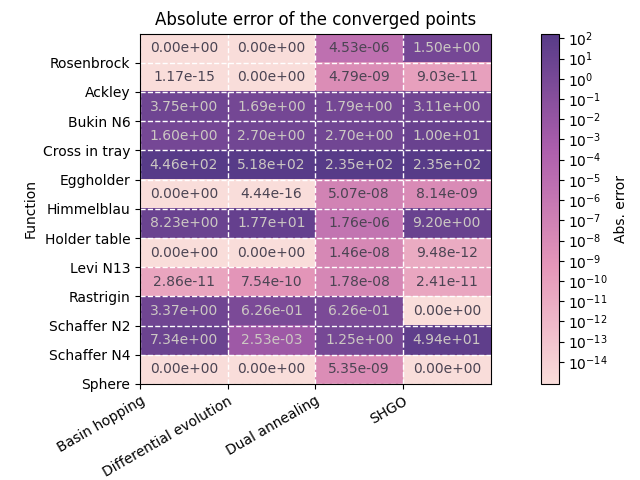
\includegraphics[width=1.2\textwidth]{../Images/error_heatmap_v4.png}
    }
    \caption{Rezultati optimizacije funkcij iz suite of benchmarks.}
    \label{fig:benchmarks_results}
\end{figure}

Vidimo, da je od vseh funkcij najbolj zoprna Eggholderjeva funkcija. Če pogledamo še na sliki (\ref{fig:benchmarks2})
vidimo, da tudi res zgleda tako. Meni se sploh ne zdi očiten tisti minimum. Pa še tako nazobčeno je vse skupaj, kar 
pomeni, da se je zelo težko znebiti lokalnih minimumov. Najlažje je pa optimizirati Sferično simetrično funkcijo,
kar je tudi zelo smiselno. V splošnem zgleda najbolj uspešna metoda kar Basin Hopping, kar se mi zdi zanimivo, da
je tako uspešna, ker v bistvu deluje na principu naključnih perturbacij. \\

\subsection{Thomsonov problem}
Verjetno najbolj zanimiv rezultat pri študiji Thomsonovega problema je slika (\ref{fig:thomson_benchmark}) kjer sem 
primerjal različne metode optimizacije. 

\begin{figure}[H]
    \centering
    \makebox[\textwidth][c]{%
    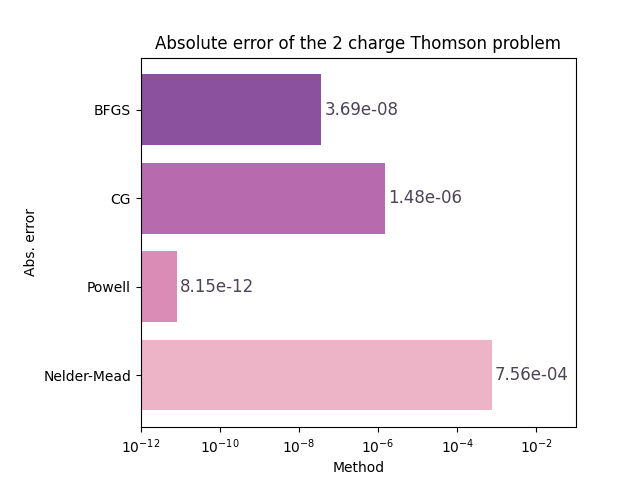
\includegraphics[width=1\textwidth]{../Images/thomson_perf1.png}
    }
    \caption{Rezultati optimizacije Thomsonovega problema za $m=1$.}
    \label{fig:thomson_benchmark}
\end{figure}

Uporabljene metode so:

\begin{itemize}
    \item BFGS - Broyden–Fletcher–Goldfarb–Shanno algorithm
    \item CG - Conjugate Gradient algorithm
    \item Powell - Powell’s conjugate direction method
    \item Nelder-Mead - Nelder-Mead simplex algorithm
\end{itemize}

Pričakoval bi, da bi bila metoda BFGS najbolj natančna zaradi tega, ker je to metoda drugega reda, ampak
izkazalo se je, da je za ta dotični primer najbolj natančna metoda Powell in to za 4 rede velikosti. Upam,
da nisem česa napačno napisal, ker se mi to zdi nekoliko nenavadno. \\

Vizualno je rešitev tega problema za nekaj različnih $m$ prikazana na sliki (\ref{fig:thomson}). \\

\begin{figure}[H]
    \centering
    \makebox[\textwidth][c]{%
    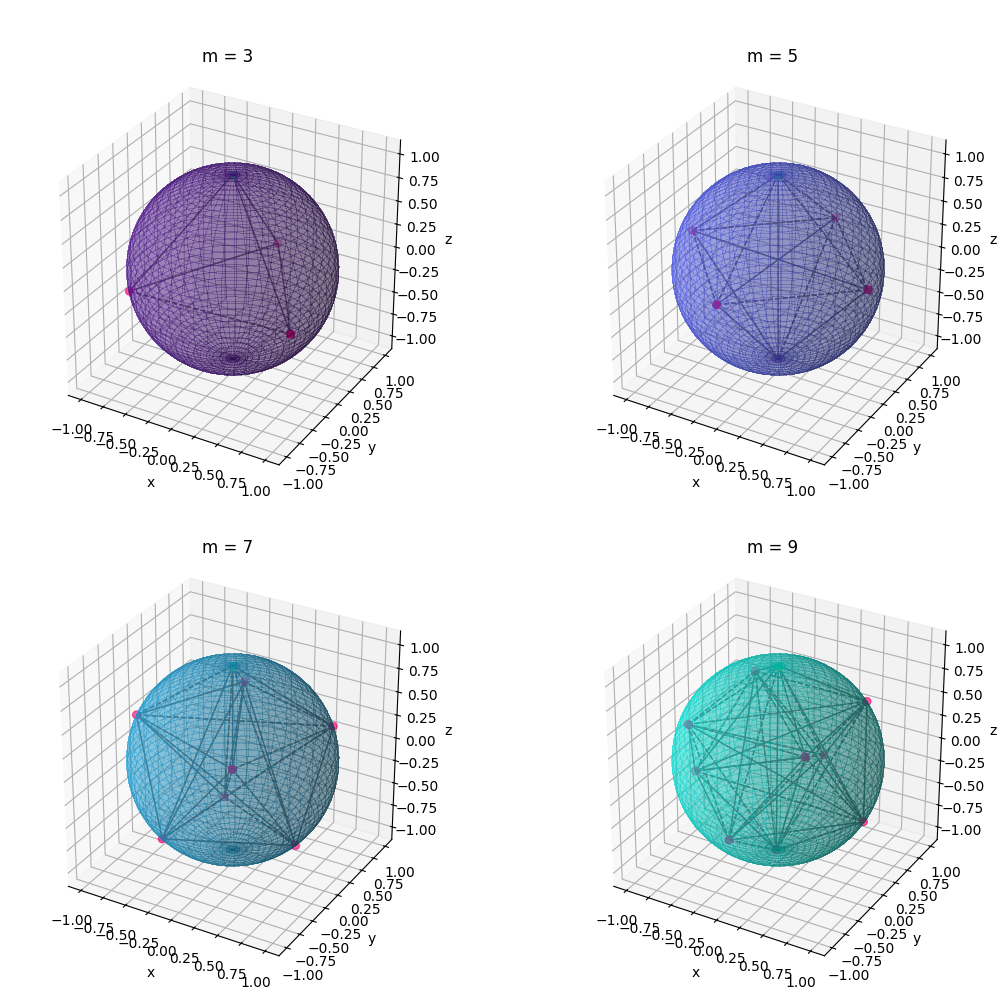
\includegraphics[width=1\textwidth]{../Images/thomson_multi.png}
    }
    \caption{Rešitev Thomsonovega problema za različne $m$.}
    \label{fig:thomson}
\end{figure}

\subsection{Vožnja skozi semafor}
Rezultati optimizacije za različne vrednosti $\kappa$ so prikazani na sliki (\ref{fig:semafor_results}). Pri vseh
rešitvah pride na koncu do neke vrste potujitve česar ne znam najbolje razložiti.

\begin{figure}[H]
    \centering
    \makebox[\textwidth][c]{%
    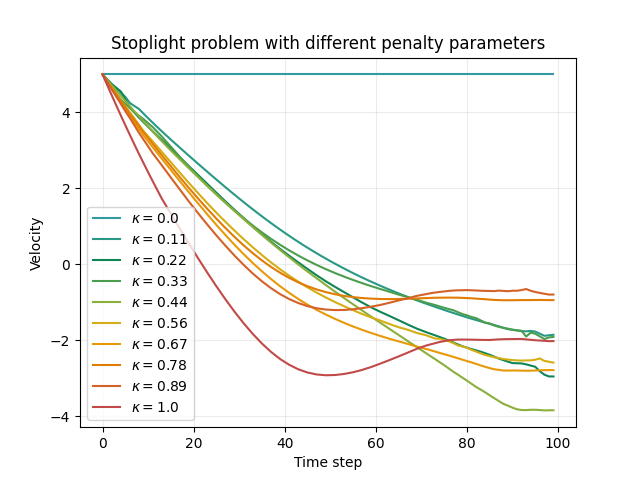
\includegraphics[width=1\textwidth]{../Images/stoplight_sweep_kappa.png}
    }
    \caption{Rezultati optimizacije za različne $\kappa$.}
    \label{fig:semafor_results}
\end{figure}

Veliko bolj praktično bi bilo, če bi jaz ta graf narisal v pravilni brezdimenzijski obliki, ampak žal nisem
utegnil. Tako je zdaj iz te slike težko razbrati, kaj se pravzaprav dogaja in s tem tudi težko primerjam 
dobljeno z rezultati prve naloge pri Modelski Analizi 1. Kot tisti drugi nov parameter od katerega so lahko 
različne rešitve sem pogledal še, kaj se spremeni ob spremembi $\Delta t$. Rezultat je prikazan na sliki 
(\ref{fig:semafor_results2}). \\

\begin{figure}[H]
    \centering
    \makebox[\textwidth][c]{%
    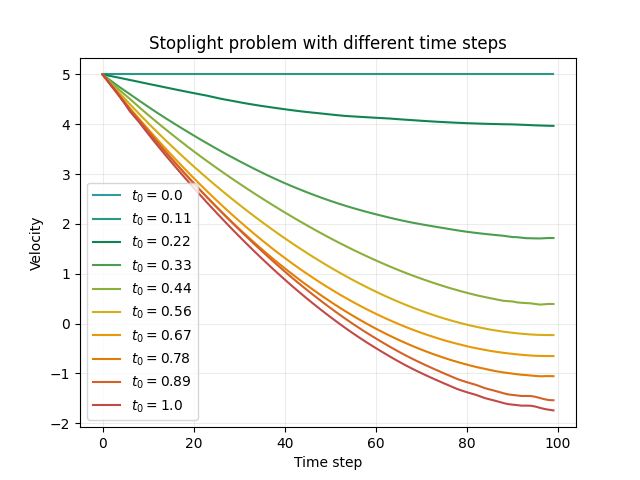
\includegraphics[width=1\textwidth]{../Images/stoplight_sweep_step.png}
    }
    \caption{Rezultati optimizacije za različne $\Delta t$.}
    \label{fig:semafor_results2}
\end{figure}

Začetna hitrost je bila tu nastavljena na $v_0 = 5$ in smiselno, če časovnega koraka ni, se nič ne spremeni. Večji 
časovni korak nam povzroči večjo spremembo hitrosti, kar pa ni vedno optimalno, ker se lahko zgodi, da postane 
hitrost negativna. To bi sicer lahko poskusil mitigirati z dodatnimi vezmi, ampak sem res želel ujeti oddajni rok in
zaradi tega sem to izpustil.

\section{Komentarji in izboljšave}
Malo sem nezadovoljen z izidom naloge, ker sem želel narediti še več, ampak žal nisem utegnil. Želel sem narediti
še več primerjav metod, še predvsem uporabo regresijskih modelov za napovedovanje optimalnih parametrov. Pravzaprav 
sem imel cel spisek stvari, ki sem jih želel narediti.. še paralelni grid search, uporaba komercialnih solverjev kot
je \texttt{gurobipy}. Na koncu mi je vse malo propadlo. Želel sem aplicirati vse to na praktičnem primeru minimizacije
višine terena Slovenije. It is what it is. \\

Najbolj se mi zdi lacking drug del naloge, kjer bi si res želel pogledati še kako vez. Morebitno kdaj dodam k tej 
nalogi še kakšen dodatek okoli tega dela, ker se mi zdi, da sem malenkost malo raziskal to področje. Je pa bilo zabavno
testirati različne metode optimizacije na različnih funkcijah. Verjetno bi si moral boljše razporediti čas, da bi lahko
naredil več. \\

\newpage
\bibliographystyle{unsrt}
\bibliography{sources}
\end{document}
